\documentclass[unicode,9pt, pdf]{beamer}
\usepackage{amsmath}
\usepackage[T2A]{fontenc}
\usepackage[utf8]{inputenc}
\usepackage[english, russian]{babel}
\usepackage{amsthm}
\usepackage{booktabs}
\usepackage{graphicx}
\usepackage{caption}
% Table float box with bottom caption, box width adjusted to content
\DeclareGraphicsExtensions{.png}
\graphicspath{{images/}}  
\usetheme{Warsaw}
\usetheme[numbers, minimal,totalnumbers,nonav]{Statmod}




\title[Deep Learning]{Deep Learning}

\author[Страшко В., Сандул М., Рукавишникова А.]{Страшко Владислав \\
        Сандул Михаил \\
        Рукавишникова Анна}
\date{
	Санкт-Петербург\\
	2019г.
}

\subject{Beamer}
\begin{document}
	
	\begin{frame}
		\titlepage
	\end{frame}
	
	\begin{frame}{Машинное обучение}
	    \begin{figure}[h]
	        \begin{center}
		        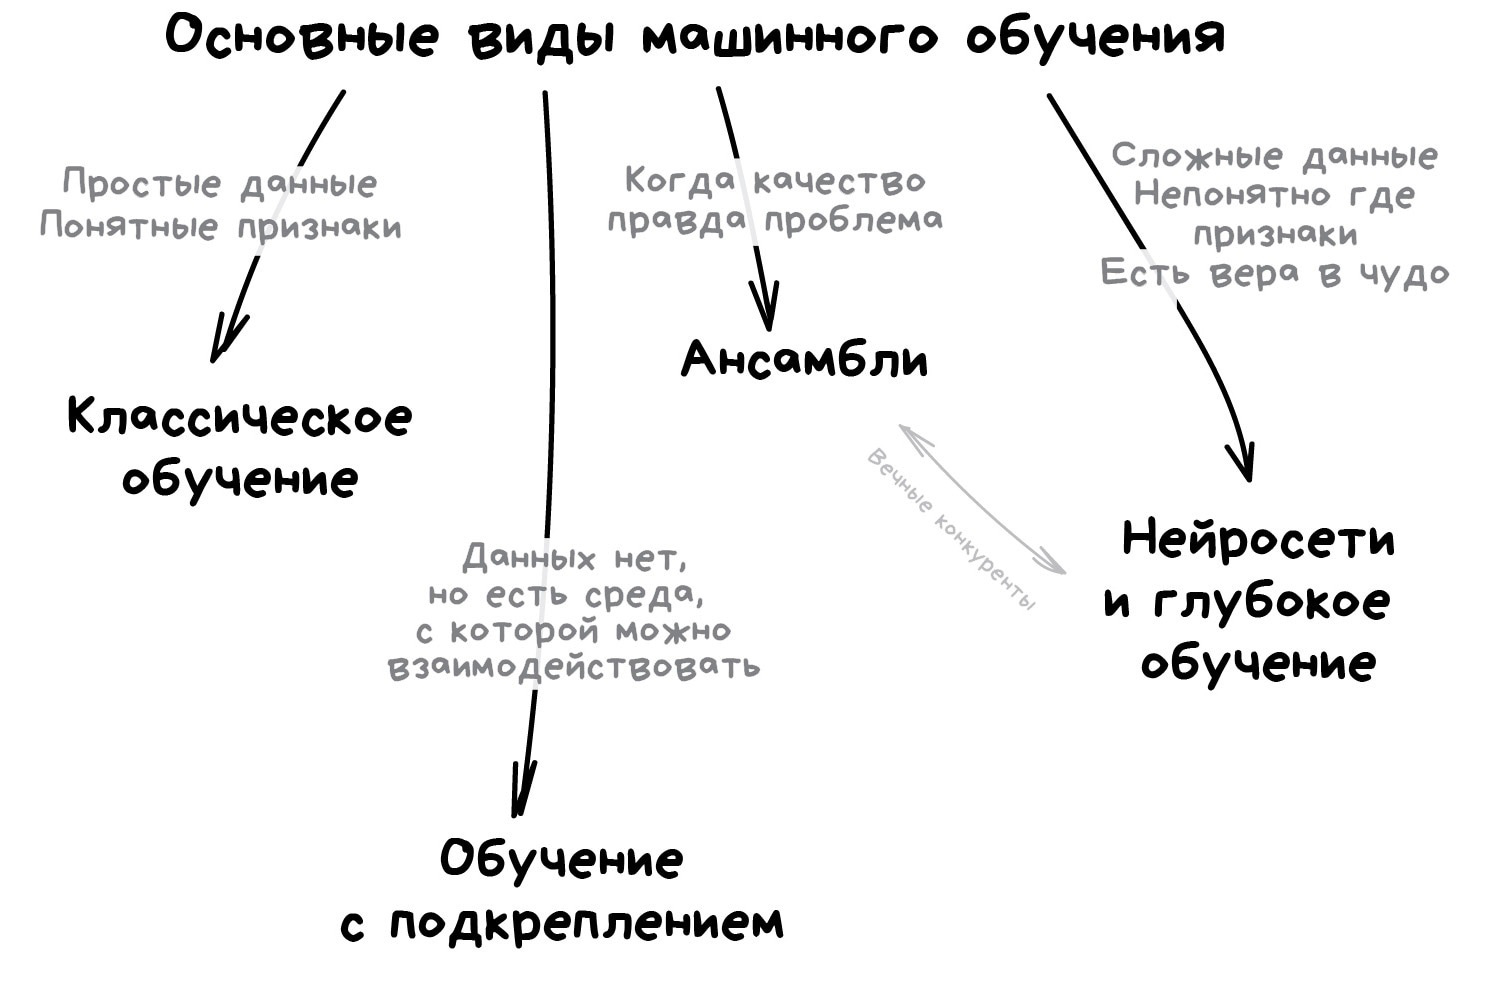
\includegraphics[width=290pt, height=150pt]{ml_pic.png}
	        \end{center}
        \end{figure}
	\end{frame}
	
	\begin{frame}{Глубокое обучение}
    \textbf{Классическое обучение:} простые данные, понятные фиксированные признаки\\
    
    \textbf{Глубокое обучение:} сложные данные, признаки метод <<выучивает>> сам\\
    \vspace{0.5cm}
	Основные представители:
        \begin{itemize}
            \item  сверточные нейронные сети (CNN): анализ изображений, текстов, речи. Обобщаются на случаи данных с некоторой локальной структурой;
            \item рекуррентные нейронные сети (RNN): обработка последовательностей векторов.
        \end{itemize}
    \vspace{0.5cm}
    Особенности:
    \begin{itemize}
        \item модель глубокого обучения собирается из большого количества блоков (сверточных, рекуррентных, полносвязных, $\ldots$);
        \item обучение на GPU (TPU)
    \end{itemize}
        
	\end{frame}
	
	\begin{frame}{ImageNet}
	    \begin{figure}
	        \centering
	        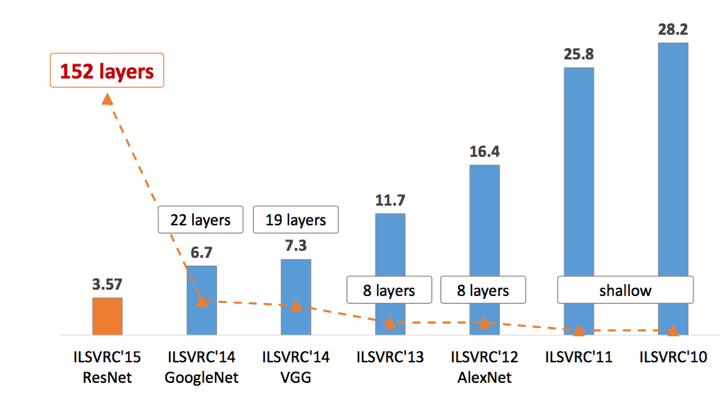
\includegraphics[width=300pt, height=150pt]{image_net.png}
	        \caption{ImageNet Classification top-5 error}
	        \label{fig:my_label}
	    \end{figure}
	\end{frame}
	
	\begin{frame}{GoogleNet}
	    \begin{figure}
	        \centering
	        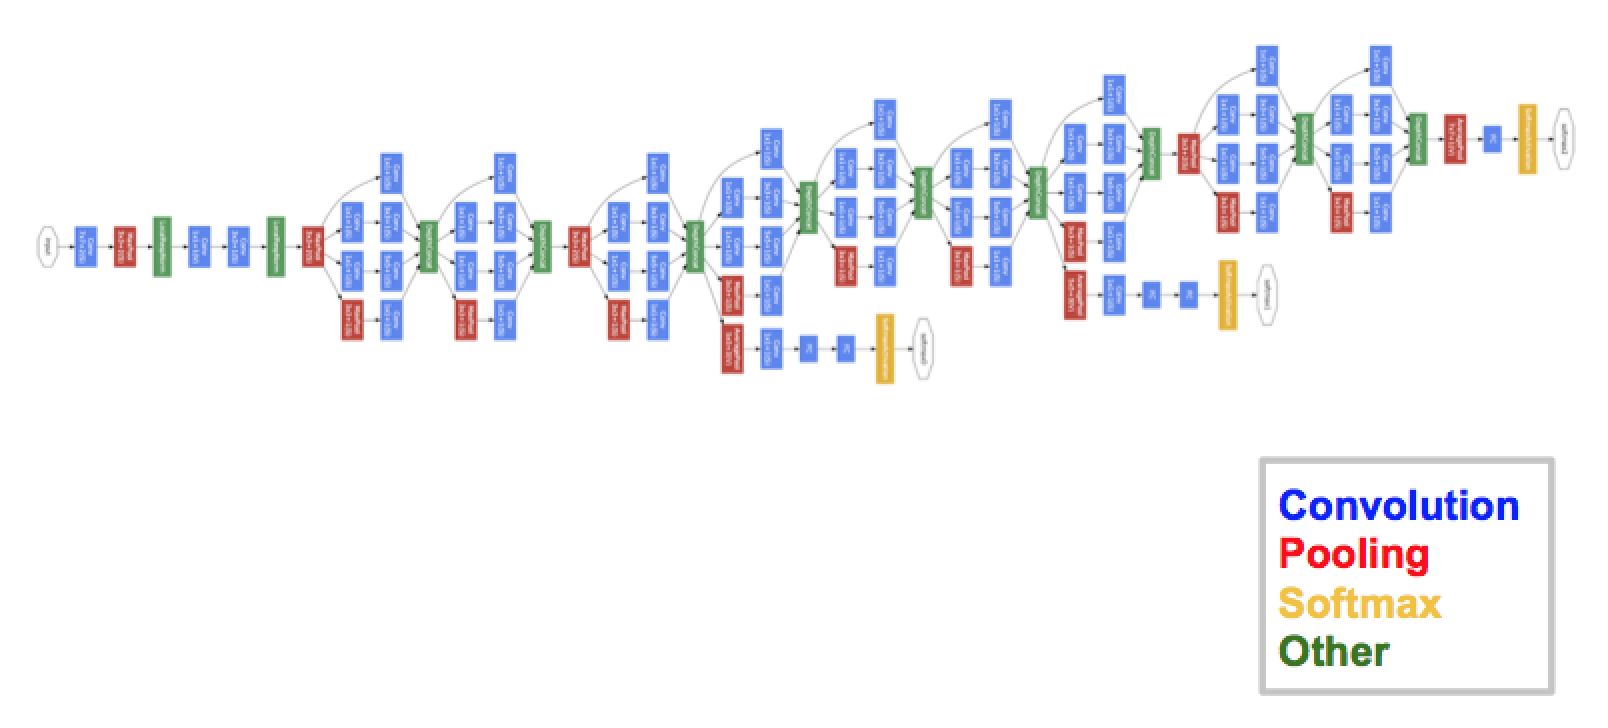
\includegraphics[width=335pt, height=200pt]{googlenet.png}
	        \caption{Архитектура GoogleNet}
	        \label{fig:my_label}
	    \end{figure}
	\end{frame}
	\begin{frame}
	    \frametitle{Рекуррентная нейронная сеть}
	    Для задачи обработки последовательностей: \\
	    \vspace{0.5cm}
	    $ x_t $ --- входной вектор в момент $ t $;\\
	    $ s_t $ --- вектор скрытого состояния в момент $t$;\\
	    $ o_t $ --- выходной вектор\\
	    \vspace{0.5cm}
	    $s_t = \sigma_s (Ux_t + Ws_{t-1})$\\
	    $o_t = \sigma_o (Vs_t)$
	    
	    \begin{figure}
	        \centering
	        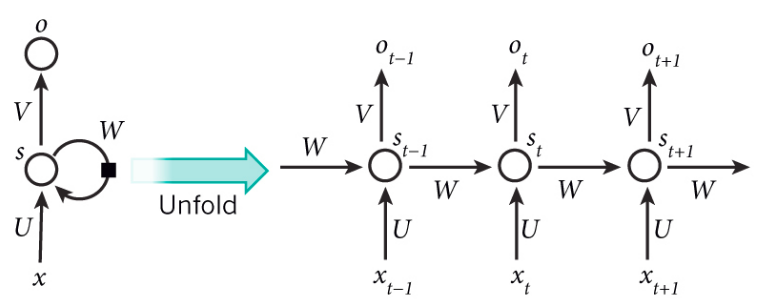
\includegraphics[width=230pt, height=90pt]{rnn.png}
	        \caption{Рекуррентная нейронная сеть}
	        \label{fig:my_label}
	    \end{figure}
	\end{frame}
	
	\begin{frame}
	\frametitle{Обучение рекуррентных сетей}
	 Обучение рекуррентной сети:
	    $$\sum_{t=0}^{T} \mathcal{L}_t (U, V, W) \rightarrow \min_{U, V, W},$$
	    где $\mathcal{L}_t (U, V, W) = \mathcal{L} (y_t(U, V, W))$ --- потеря от предсказания $y_t$\\
	\vspace{0.5cm}
	Специальный вариант обратного распространения ошибок, \\
	Backpropagation Through Time (BPTT): \\
	$$\dfrac{\partial \mathcal{L}_t}{\partial W} = \dfrac{\partial \mathcal{L}_t}{\partial o_t} \dfrac{\partial o_t}{\partial s_t} \sum_{k=0}^t \left( \prod_{i = k + 1}^t \dfrac{\partial s_i}{\partial s_{i-1}} \right) \dfrac{\partial s_k}{\partial W}$$
	Здесь есть 2 проблемы:
	\begin{enumerate}
	    \item нам не нужно помнить всю историю --- можем считать только несколько последних скрытых состояний\\
	    \item Затухание/взрыв градиентов, если  $\frac{\partial s_i}{\partial s_{i-1}} \not\rightarrow 1$ --- ограничить частную производную(ввести архитектуру, чтобы эта величина стремилась к 1)
	\end{enumerate}

    \end{frame}
    
    \begin{frame}{LSTM (long short-term memory)}
        Мотивация LSTM: сеть должна долго помнить контекст, какой именно --- сеть должна выучить сама. Поэтому вводится $C_t$ --- вектор состояния сети в момент $t$.\\
        
        \begin{figure}[h]
	\begin{center}
		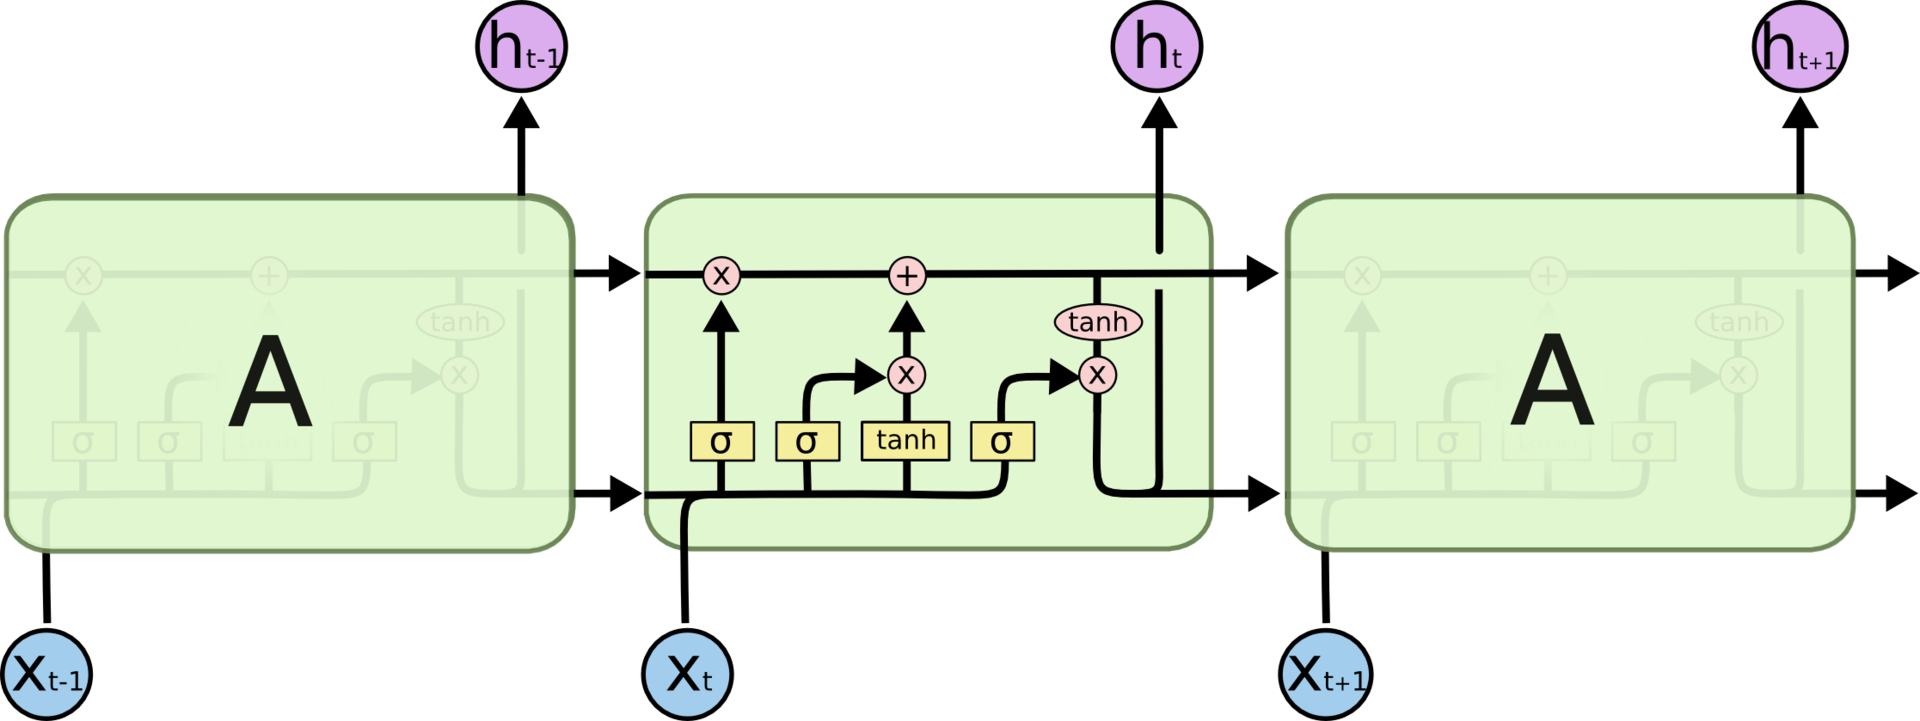
\includegraphics[width=280pt, height=100pt]{lstm.png}
	\end{center}
\end{figure}
        \begin{figure}[h]
	\begin{center}
		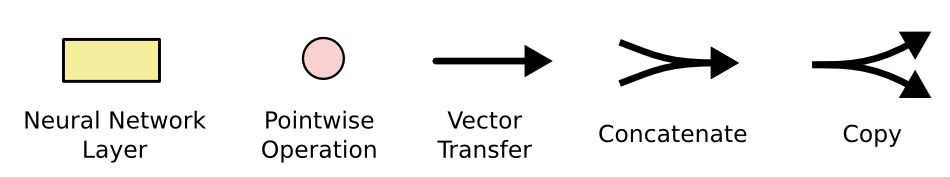
\includegraphics[width=280pt, height=70pt]{lstm_signs.png}
	\end{center}
\end{figure}
        \end{frame}
	
	\begin{frame}{LSTM (long short-term memory)}
	    \begin{figure}[h]
	        \begin{center}
		        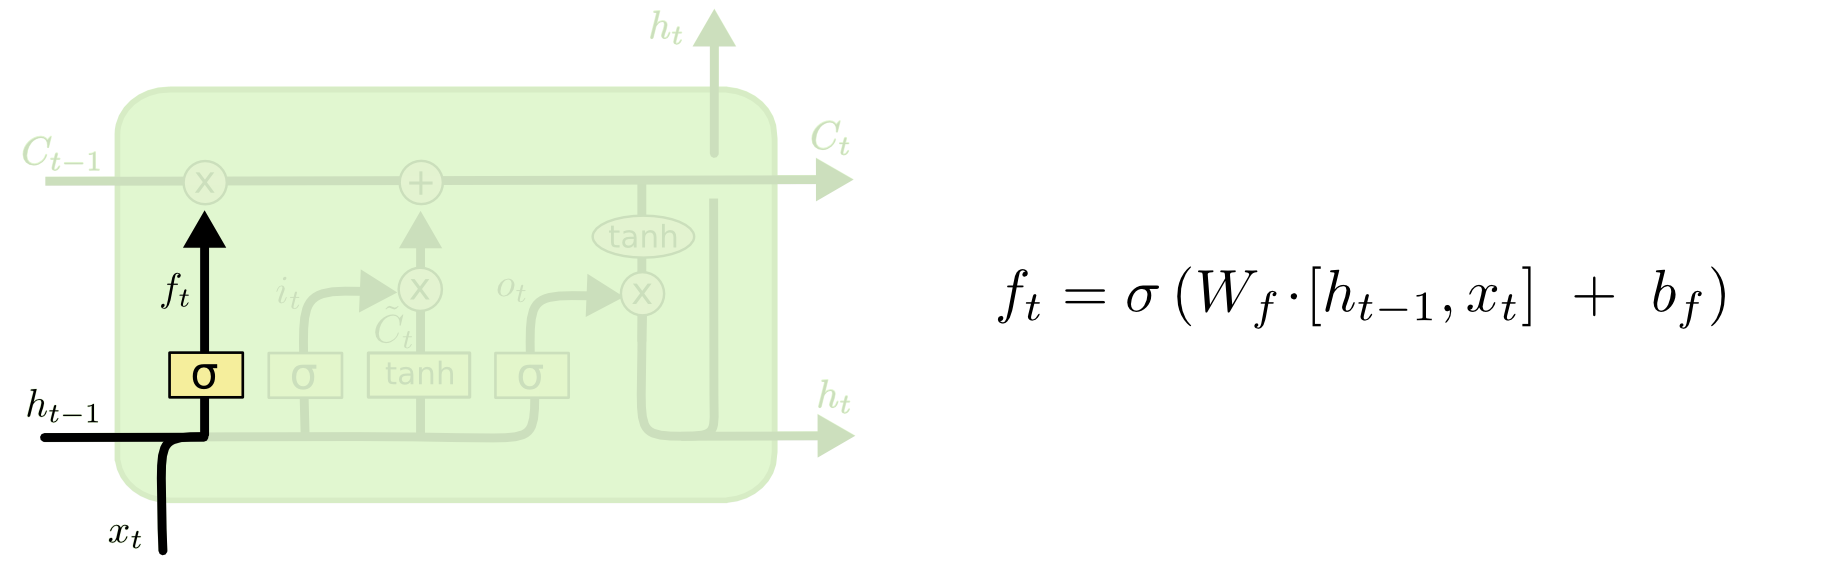
\includegraphics[width=280pt, height=100pt]{lstm_forget_gate.png}
	        \end{center}
        \end{figure}
        Фильтр забывания (forget gate) c параметрами $W_f$, $b_f$ решает, какие координаты вектора состояния $C_{t-1}$ надо запоминать.\\ Своего рода <<классификатор>>. \\
        Здесь $\sigma$ --- сигмоида.
	\end{frame}
	\begin{frame}{LSTM}
	    \begin{figure}[h]
	        \begin{center}
		        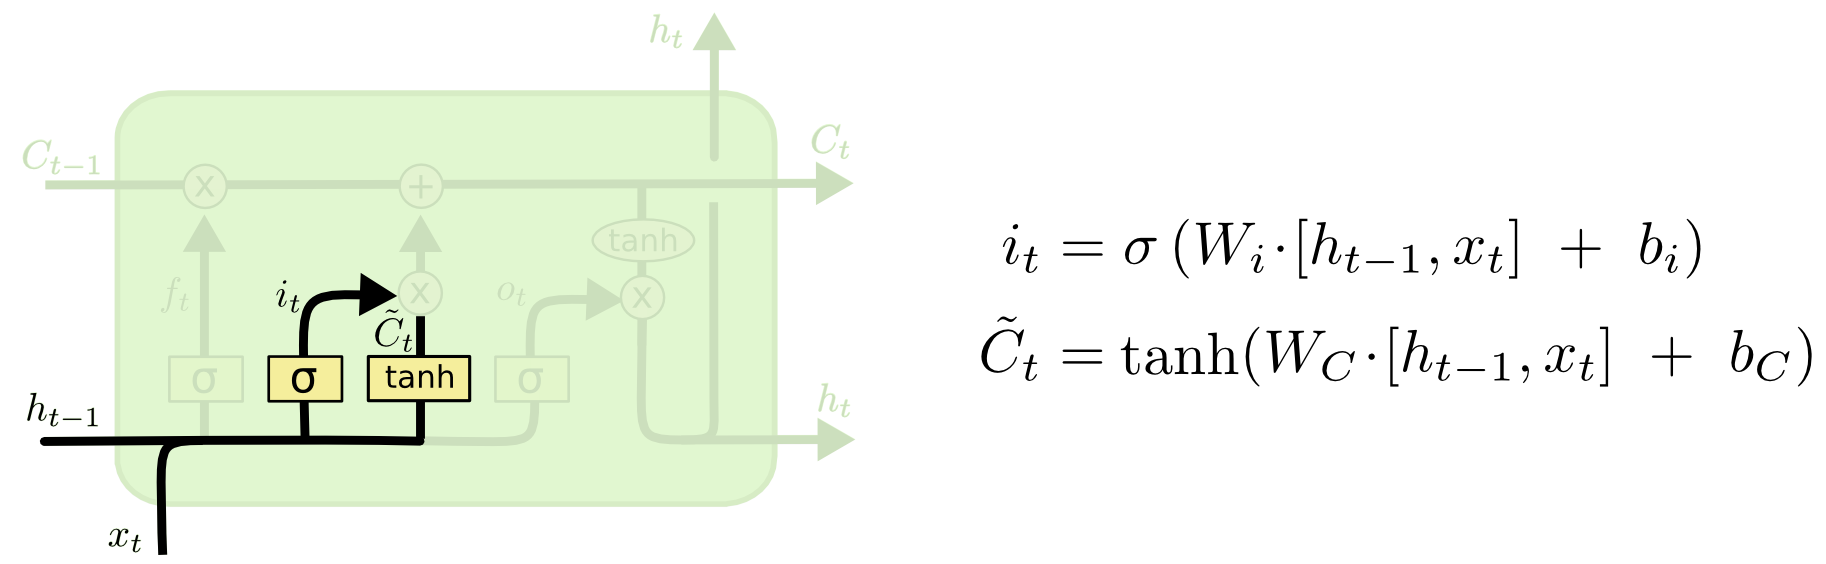
\includegraphics[width=280pt, height=100pt]{input_layer_gate.png}
	        \end{center}
        \end{figure}
        Фильтр входных данных (input gate) с параметрами $W_i$, $b_i$ решает, какие координаты вектора состояния надо обновить. \\
        \vspace{0.5cm}
        Модель нового состояния с параметрами $W_C,$ $b_C$ формирует вектор $\widetilde{C}_t$ значений-кандидатов нового состояния.
	\end{frame}
	\begin{frame}{LSTM (long short-term memory)}
	    \begin{figure}[h]
	        \begin{center}
		        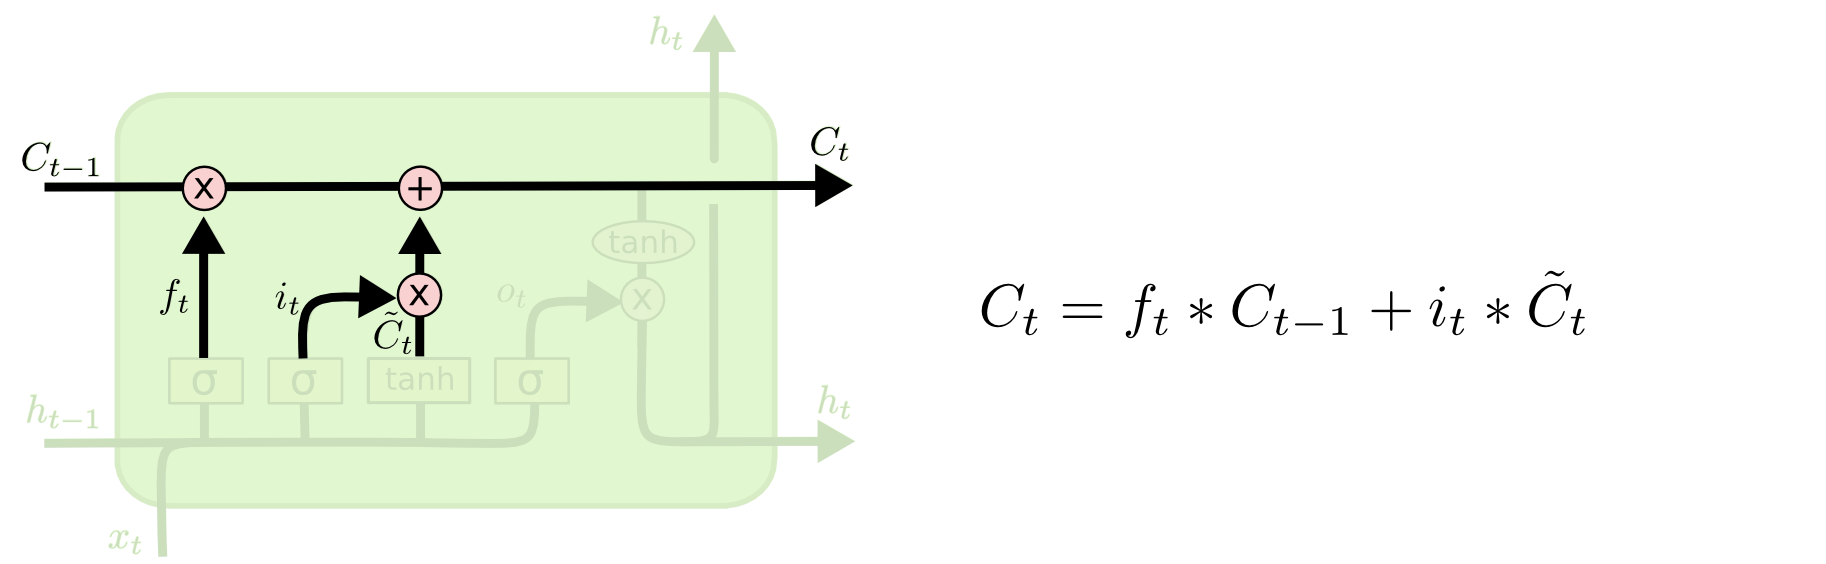
\includegraphics[width=280pt, height=100pt]{lstm_state.png}
	        \end{center}
        \end{figure}
    Новое состояние $C_t$ формируется как смесь старого состояния $C_{t-1}$ с фильтром $f_t$ и вектора значений-кандидатов $\widetilde{C}_t$ с фильтром $i_t$.\\
    Здесь операция покоординатного умножения. \\
    \vspace{0.5cm}
    Обучаемых параметров нет.
	\end{frame}
	
	\begin{frame}{LSTM}
	    \begin{figure}[h]
	        \begin{center}
		        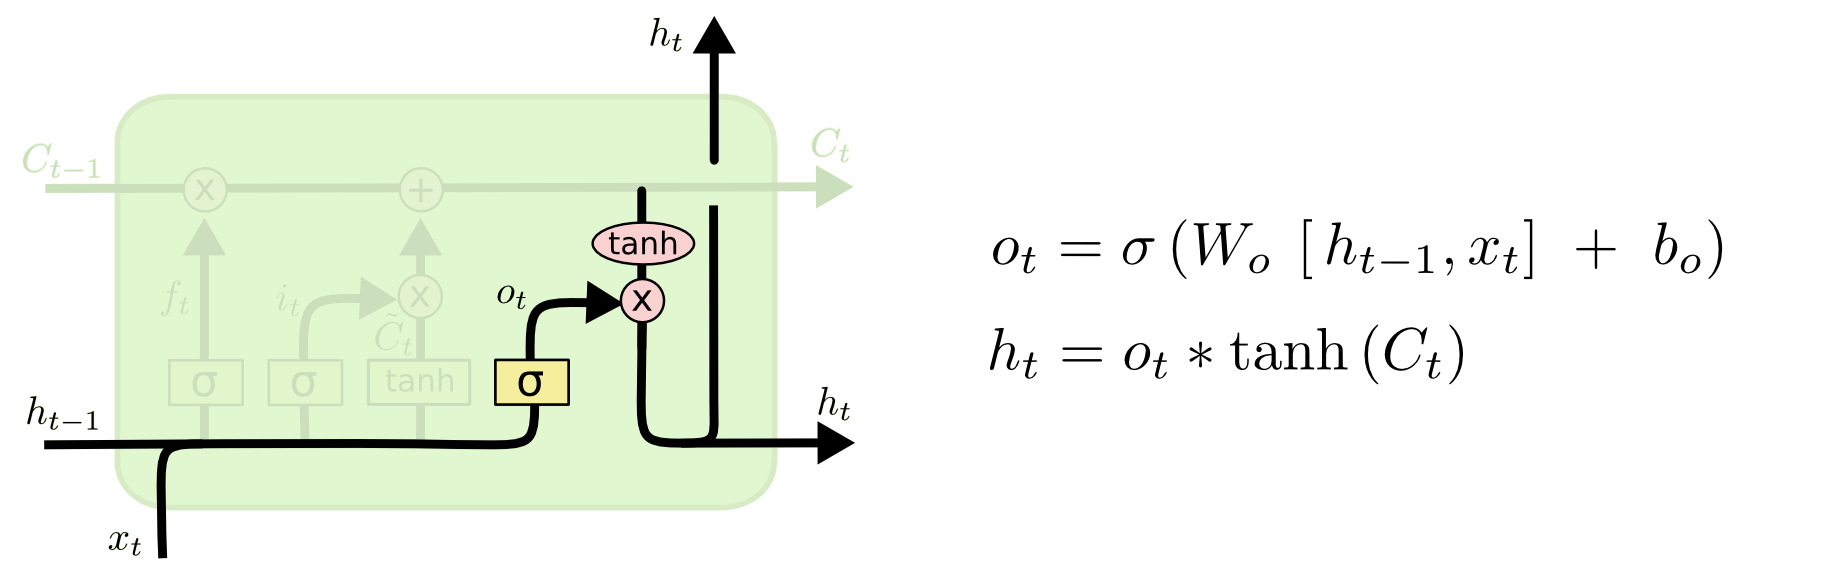
\includegraphics[width=280pt, height=100pt]{lstm_out.png}
	        \end{center}
        \end{figure}
        Фильтр выходных данных (output gate) с параметрами $W_o, b_o$ решает, какие координаты вектора состояния $C_t$ надо учесть. 
        \vspace{0.5cm}
        Выходной сигнал $h_t$ формируется из вектора состояния $C_t$ с помощью нелинейного преобразования th и фильтра $o_t$.
	\end{frame}
	
	\begin{frame}{LSTM с <<замочными скважинами>>}
	    \begin{figure}[h]
	        \begin{center}
		        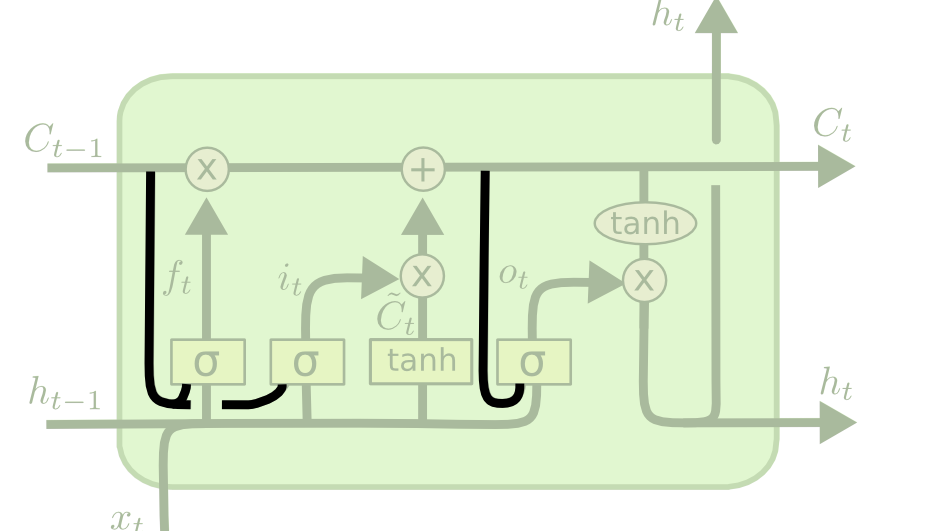
\includegraphics[width=280pt, height=100pt]{lstm_peepholes.png}
	        \end{center}
        \end{figure}
        Здесь в каждом слое сети учитываются вектора состояния $C_t$ и $C_{t-1}$.
	\end{frame}
	
\begin{frame}{LSTM: Gated Recurrent Unit (GRU)}
    \begin{figure}[h]
	        \begin{center}
		        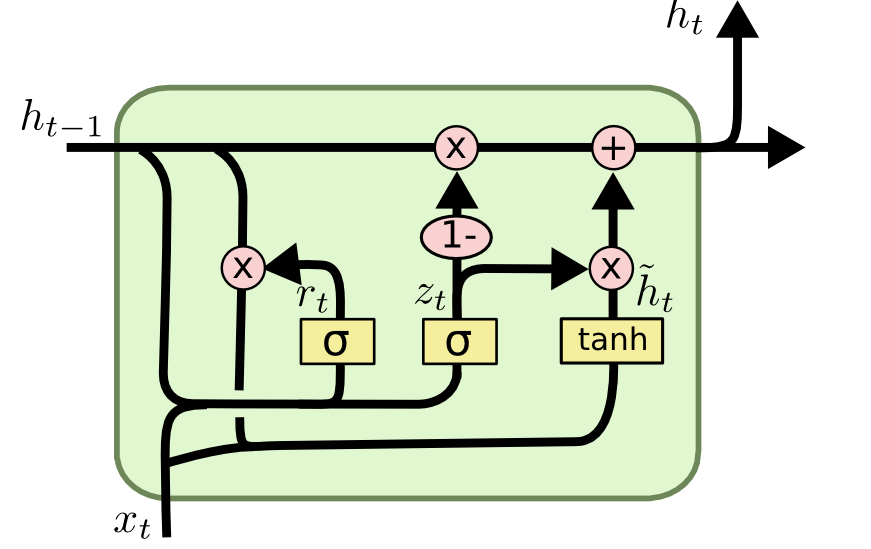
\includegraphics[width=280pt, height=100pt]{lstm_gru.png}
	        \end{center}
        \end{figure}
        Используется только состояние $h_t$, вектора $C_t$ нет. \\
        $z_t$ вместо входного и забывающего фильтров.\\
        Фильтр перезагрузки $\widetilde{h}_t$ решает, какую часть памяти нужно перенести дальше с прошлого шага.\\
        
\end{frame}

\begin{frame}{Применение к временным рядам}
    \textbf{Прогноз при помощи сетей прямого распространения}:
        \begin{itemize}
            \item проходим окном длины $L$ вдоль ряда, каждое окно --- $L$-мерный элемент обучающей выборки
            \item в качестве входного слоя используем $L$ последних наблюдений ряда, в качестве выходного --- значение прогноза на 1 точку вперед
        \end{itemize}
    \textbf{Рекуррентные сети:}
    \begin{itemize}
        \item RNN --- архитектура one-to-many  
        \item предыдущий выход переиспользуется для предсказания на несколько точек. Частный случай --- one-to-one
    \end{itemize}
    \begin{figure}
        \centering
        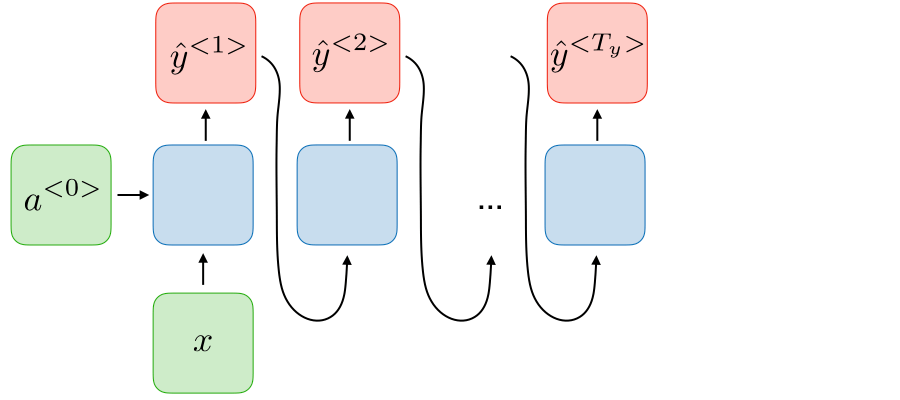
\includegraphics[width=320pt, height=100pt]{rnn-one-to-many.png}
        \caption{RNN: One to many}
        \label{fig:my_label}
    \end{figure}
\end{frame}

\begin{frame}{Векторное представление объектов}
    Рекуррентная нейронная сеть принимает на вход вектора. Нужно каким-то образом вложить объекты в векторное пространство.\\
    \vspace{0.5cm}
    Word embeddings --- семейство методов представления слов естественного языка в виде векторов \\
    \vspace{0.5cm}
		Желаемый результат вложения:
		\begin{itemize}
			\item  Близкие вектора в смысле расстояния соответствуют семантически/синтаксически близким словам.\\
			
			\item Свойство аналогии слов: $ \text{King} - \text{Man} = \text{Queen} - \text{Woman} $
 		\end{itemize}
 		\begin{block}{word2vec}
 		    Модель: вероятность слова $w$ быть в контексте слова $u$:
 		    $$p(w|u) = \dfrac{\exp <x_w, x_u>}{\sum_v \exp<x_v, x_u>}$$
 		    Оценка максимального правдоподобия:
 		    $$\sum_{w,u \in W} n_{wu} \log p(w|u) \rightarrow \max_{x_w},$$ где $n_{wu}$ --- частота совместной встречаемости слов $u$ и $w$
 		\end{block}
\end{frame}
	

\end{document}

